\section{Observation, data analysis and methods}

    \subsection{Data selection}
        %selection criteria of scw: sun activity, elongation and presence of scw
        Given that Venus was never purposedly targeted by any of the \textit{INTEGRAL} instruments, the idea was to scan the different science windows (scw) of the
        telescope corresponding to the planet's position in the sky at that moment. Many scw fulfill this condition. Given that planets emit mostly in the softer range
        of the X-ray spectra, only JEM-X data was used. To ensure the best data quality, other criteria 
        were applied in the data selection. First, scw with increased sun activity were targeted. The sun regained activity following its 11 years cycle in 2021. 
        The April and May 2022 months, with an increase in $\sim$ 79\% and 107\% were appropriate. The elongation of Venus with respect to Earth and the telescope
        were also an important criteria. The elongation represents the Sun-Earth-Venus angle. When the angle is too small, Venus is by construction close to the Sun in the telescope's FoV and hence unobservable(and unobserved by the telescope anyway). \textbf{Fig.} \ref{elongation} illustrates the concept of elongation and \textbf{Fig.} \ref{venus_pos} shows Venus' position during the month of April 2022.

    \begin{figure}[H]
        \centering
        
\includegraphics[width = 12cm]{report/Figures/methods/Positional_astronomy.png}
        \caption{Heliocentric diagram of the positional representation of the Earth with respect to inner and outer planets. The greatest elongation is the $\alpha$ angle. It represents the Sun-Earth-Planet angle and is only shown for an outer planet on this diagram.}
        \label{elongation}
    \end{figure}
    
    \begin{figure}[H]
        \centering
        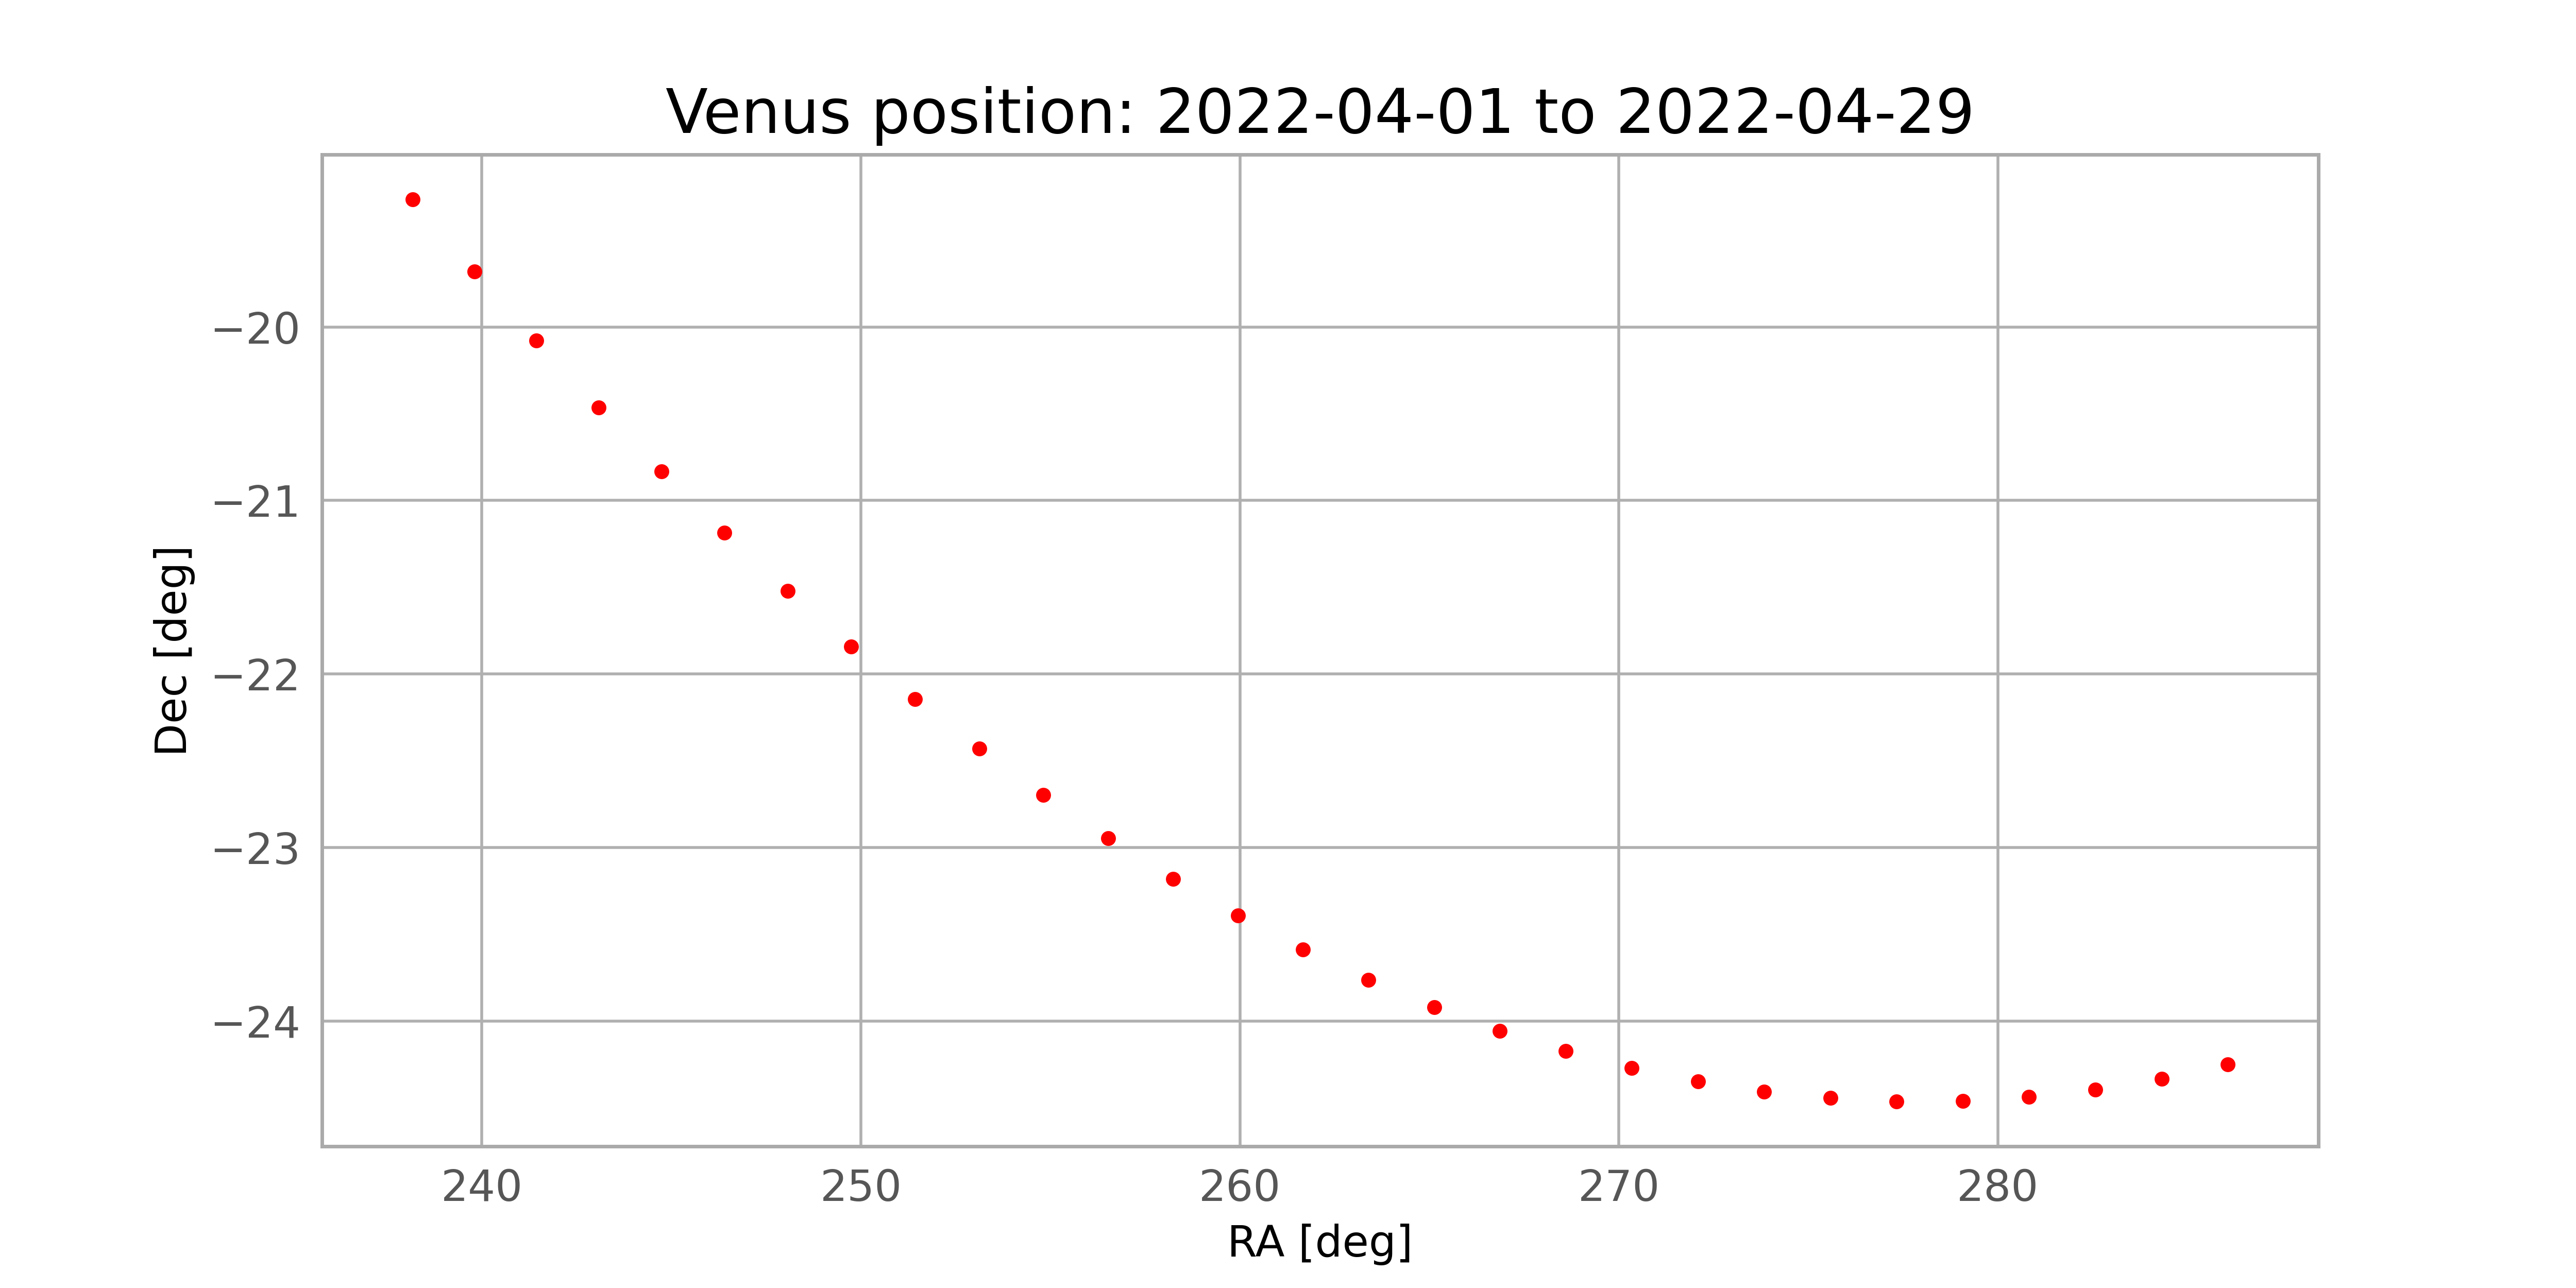
\includegraphics[width = 12cm]{report/Figures/methods/Venus_position.png}
        \caption{Position of Venus every day in the ICRF between the 01.04.2022 and 29.04.2022.}
        \label{venus_pos}
    \end{figure}

        The query was made with the \texttt{ODA-API} given the criteria above and following the parameters listed below:
        \begin{lstlisting}[language = Python,caption = Query parameters template used for both dates.,label = dict]
        par_dict = {
        "E1_keV": "3",
        "E2_keV": "10",
        "detection_threshold": "5",
        "instrument": "jemx",
        "osa_version": "OSA11.2",
        "product": "jemx_image",
        "product_type": "Real",
        "scw_list": scw_list,
        "integral_data_rights": "all-private",#all-private or public
        "token": token
        }
        \end{lstlisting}
        %put some python code, listing with jemx2(radius, energy range etc...) query.
        Quoting \cite{2020ISDCManual}: \textit{In practice, the transmission of the collimator beyond an off-axis angle of 5° is so low that only the very brightest sources can be observed at larger angles}. Therefore,

        The only scws satisfying these criteria were found in April 2022: four on the 18th, two on the 20th, fourteen on the 22nd and six on the 24th. 
        The data of the 18th and the 20th were eventually not used due to Venus being too excentered in the image. Some scws from the 22nd and 24th were discarded for
        the same reasons.  A summary of all final scws used is shown on \textbf{Tab.} ??. The characteristics of Venus in the 22.04.2022 to 24.04.2022 are shown on 
        \textbf{Tab.} ??.
        %put characteristics of venus on 22 and 24, put apparent size, pixel size, illumination, elongation, is it approaching or leaving, etc...
        \begin{table}[H]
        \centering
        \begin{tabular}{@{}ccccccc@{}}
        \toprule
        Date                         & scw\textunderscore id       & Time (UTC)          & Elongation [°] & Apparent size [''] & Illumination [\%] & $\Delta$ [AU] \\ \midrule
        \multirow{11}{*}{22.04.2022} & 249400200010 & 04:12:03 - 04:45:23 & 43.88          & 17.89              & 64.30            & 0.93          \\
         & 249400210010 & 04:47:45 - 05:20:55 & 43.88 & 17.89 & 64.31 & 0.93 \\
         & 249400220010 & 05:22:52 - 05:56:13 & 43.88 & 17.89 & 64.32 & 0.93 \\
         & 249400230010 & 05:58:34 - 06:31:43 & 43.87 & 17.88 & 64.33 & 0.93 \\
         & 249400240010 & 06:33:55 - 07:07:14 & 43.87 & 17.88 & 64.34 & 0.93 \\
         & 249400250010 & 07:09:37 - 07:42:45 & 43.87 & 17.88 & 64.34 & 0.93 \\
         & 249400260010 & 07:44:42 - 08:18:03 & 43.85 & 17.87 & 64.35 & 0.93 \\
         & 249400270010 & 08:20:27 - 08:53:35 & 43.85 & 17.87 & 64.36 & 0.93 \\
         & 249400310010 & 10:41:30 - 11:14:50 & 43.85 & 17.87 & 64.37 & 0.93 \\
         & 249400320010 & 11:17:16 - 11:50:21 & 43.84 & 17.87 & 64.37 & 0.94 \\
         & 249400330010 & 11:52:20 - 12:25:41 & 43.84 & 17.86 & 64.38 & 0.94 \\ \midrule
        \multirow{4}{*}{24.04.2022}  & 249500240010 & 19:47:17 - 20:20:27 & 43.50          & 17.52              & 65.33            & 0.95          \\
         & 249500250010 & 20:22:48 - 20:55:58 & 43.49 & 17.51 & 65.34 & 0.95 \\
         & 249500260010 & 20:58:10 - 21:31:29 & 43.49 & 17.51 & 65.35 & 0.95 \\
         & 249500270010 & 21:33:27 - 22:06:47 & 43.48 & 17.50 & 65.36 & 0.95 \\ \midrule 
        \end{tabular}
        \caption{Journal of observations and parameters.
        scw\textunderscore id: science window identifier, $\Delta$: distance from INTEGRAL, Ilumination: fraction of Venus illuminated as seen from observer computed at the beginning of each scw.}
        \label{journal}
        \end{table}



    A nothworthy aspect of targeting an object such as a planet with this telescope is that it moves in the integrated image. Scws last usually between 30min and 1 hour and 
    this is enough for Venus to move in the image of about 1 to 2 pixels.
    
    \paragraph{22.04.2022 data}

    The April 22 data consists of...
    
    \textbf{Fig.} \ref{22_map_single} shows ...
    

        \begin{figure}[H]
        \centering
        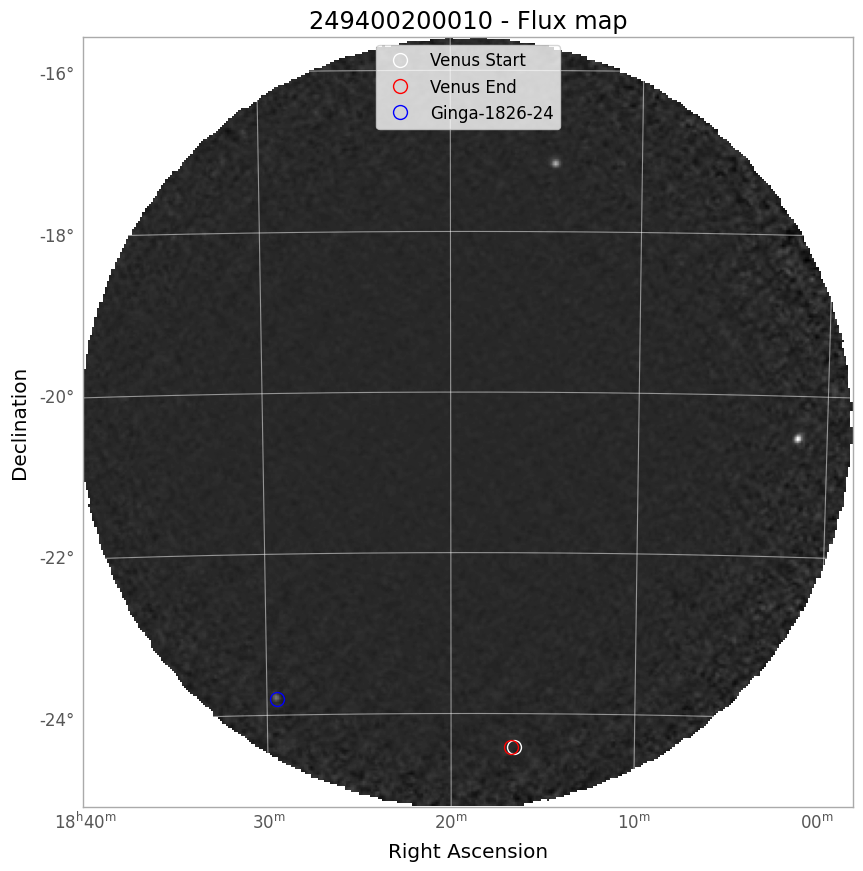
\includegraphics[width = 8cm]{report/Figures/methods/2204/20_map.png}
        \caption{Flux map from the first scw where Venus is present on the 22.04.2022. The start and end positions of Venus are circled in white and red respectively. Another bright source is also to verify the correct localisation approach.}
        \label{22_map_single}
        \end{figure}

        \begin{figure}[H]
        \centering
        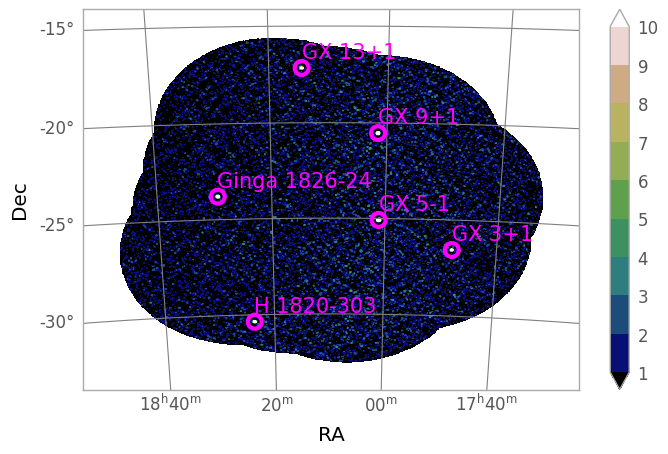
\includegraphics[width = 12cm]{report/Figures/methods/2204/oda_2204.png}
        \caption{Mosaic made with the precedent images using the \texttt{ODA} plot tools for the 22.04.2022 data.}
        \label{22_mosaic}
        \end{figure}
    
    \paragraph{24.04.2022 data}
    The April 24 data consists of ...

        \begin{figure}[H]
        \centering
        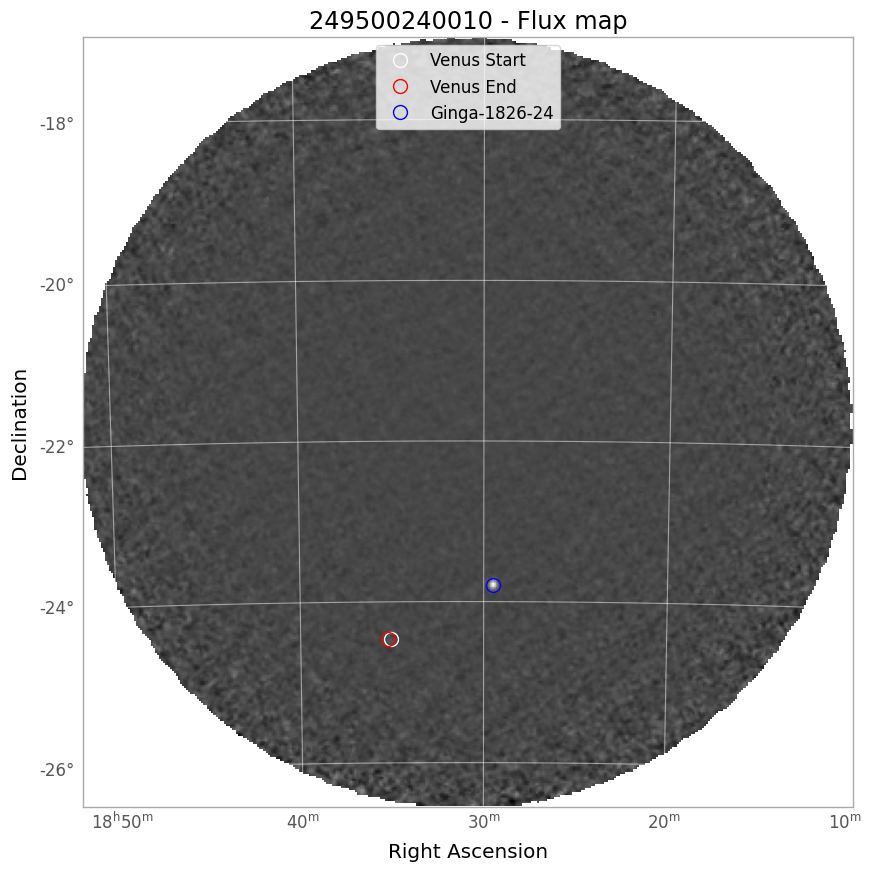
\includegraphics[width = 8cm]{report/Figures/methods/2404/24_map.png}
        \caption{Flux map from the first scw where Venus is present on the 24.04.2022. The start and end positions of Venus are circled in white and red respectively. Another bright source is also to verify the correct localisation approach.}
        \label{24_map_single}
        \end{figure}


        \begin{figure}[H]
        \centering
        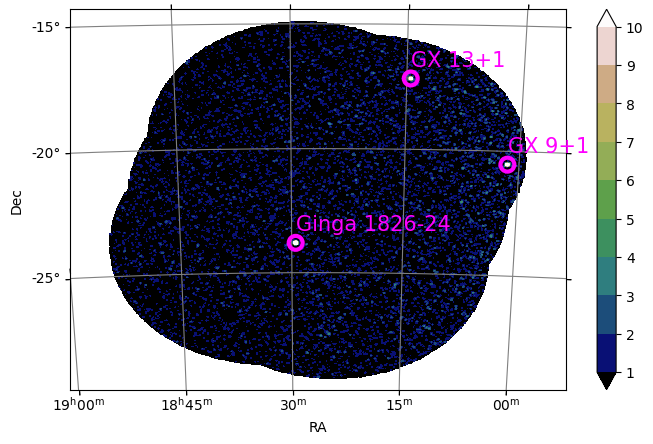
\includegraphics[width = 12cm]{report/Figures/methods/2404/oda_2404.png}
        \caption{Mosaic of the 24.04.2022 data.}
        \label{24_mosaic}
        \end{figure}

    
    \subsection{Models and assumptions}

        \begin{figure}[H]
        \centering
        \begin{subfigure}{.45\textwidth}
            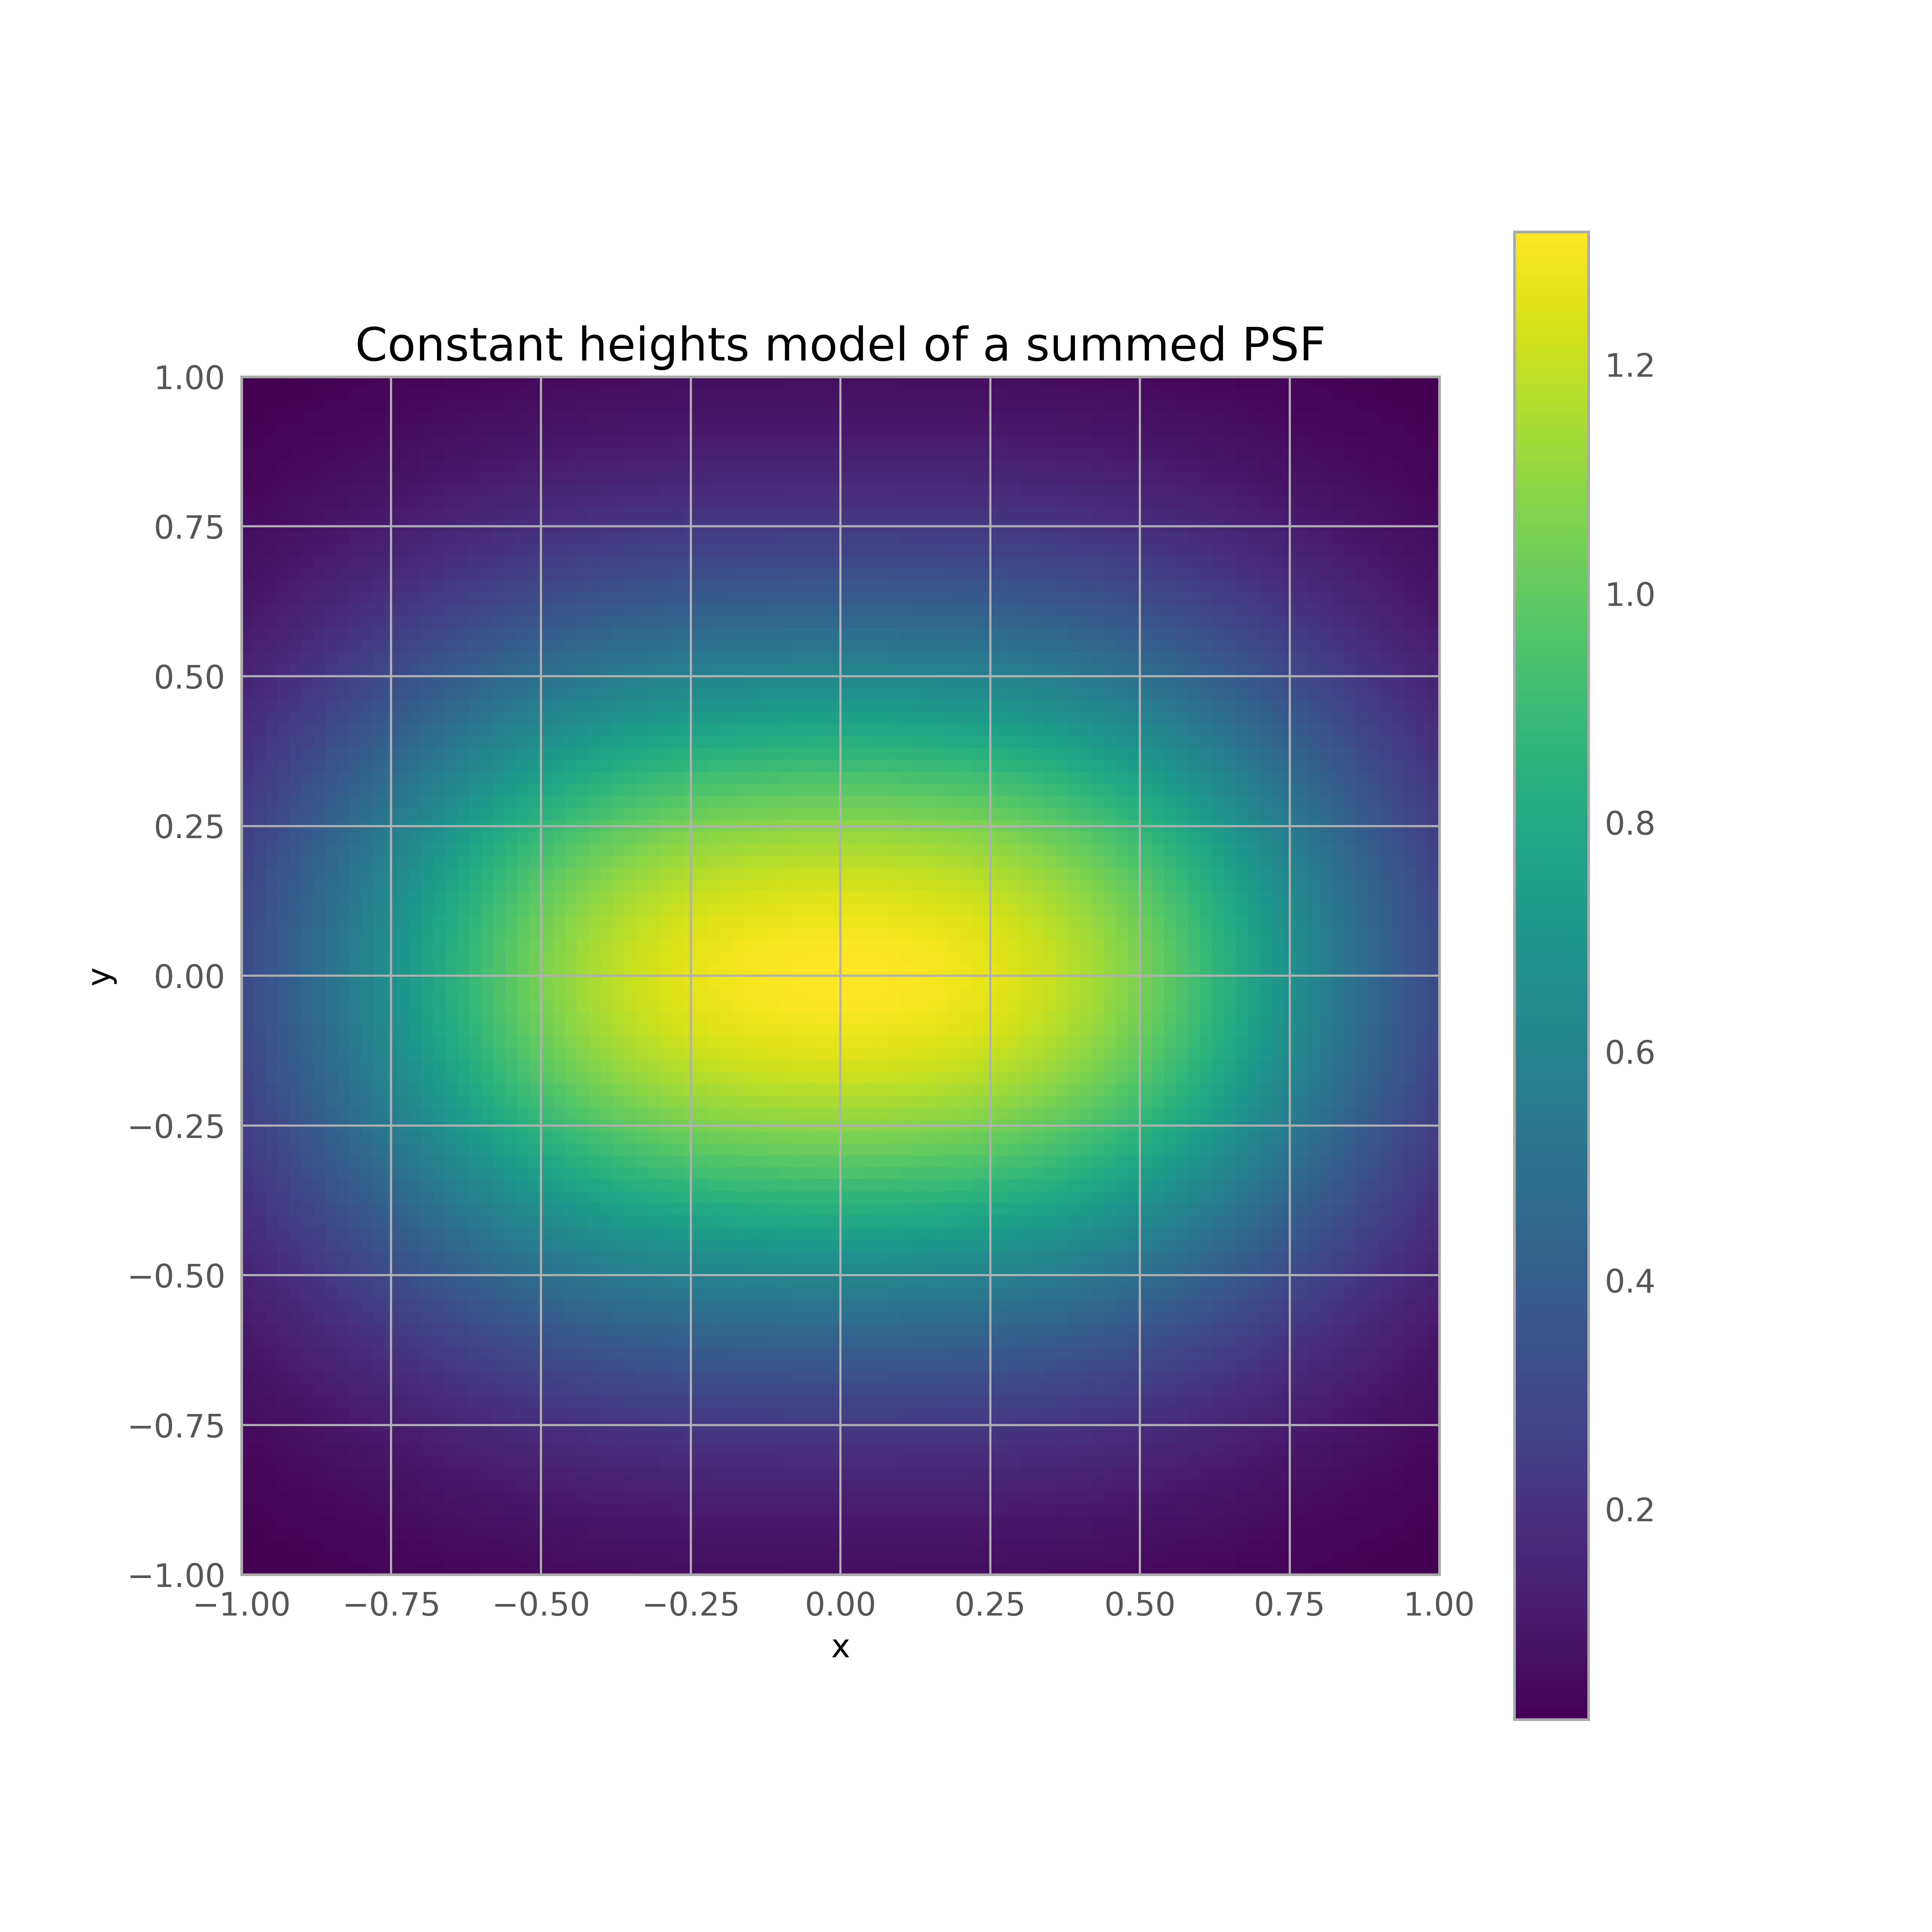
\includegraphics[width=\textwidth]{report/Figures/models/model_psf_const.png}
        \end{subfigure}%
        \hspace{1em}-
        \begin{subfigure}{.45\textwidth}
            \centering
            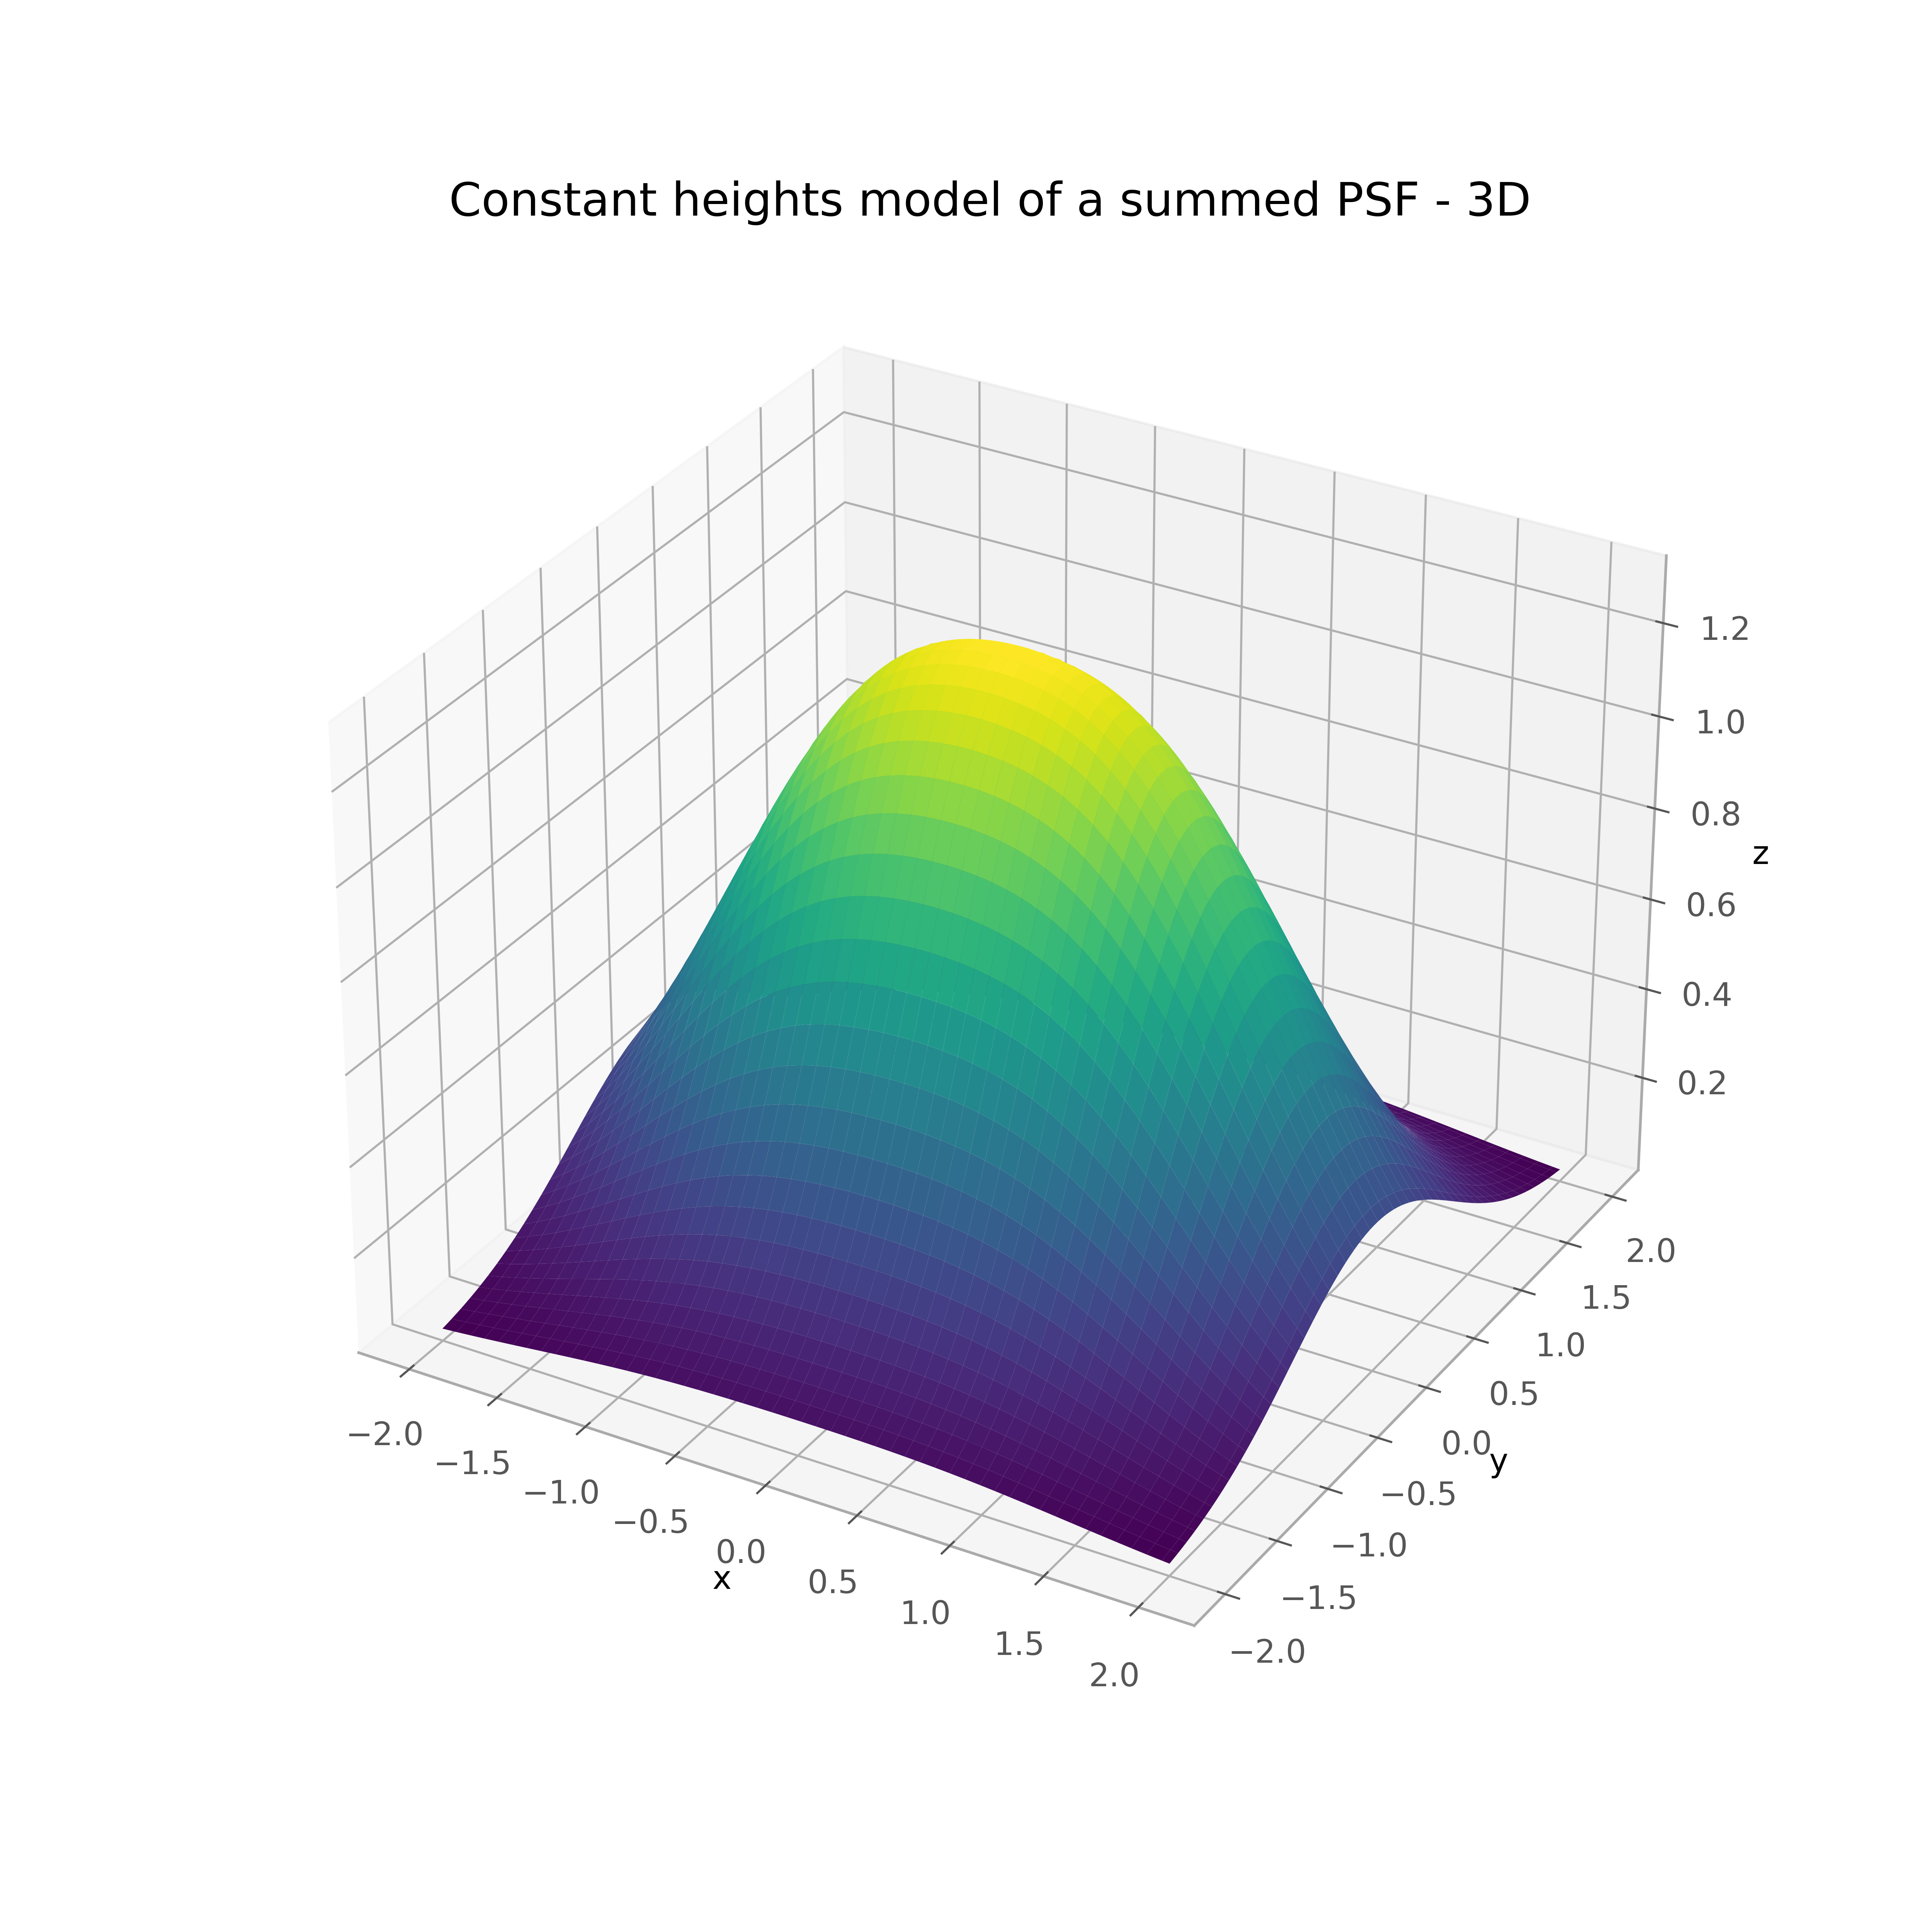
\includegraphics[width=\textwidth]{report/Figures/models/model_psf_const_3d.png}
        \end{subfigure}
        \caption{Constant summed PSFs used as models for Venus' flux.}
        \label{model_psf_const}
        \end{figure}


        %explain here why it's relevant to have a psf not const: because the time variability of venus can be of order of venus(see chandra paper).


        \begin{figure}[H]
        \centering
        \begin{subfigure}{.45\textwidth}
            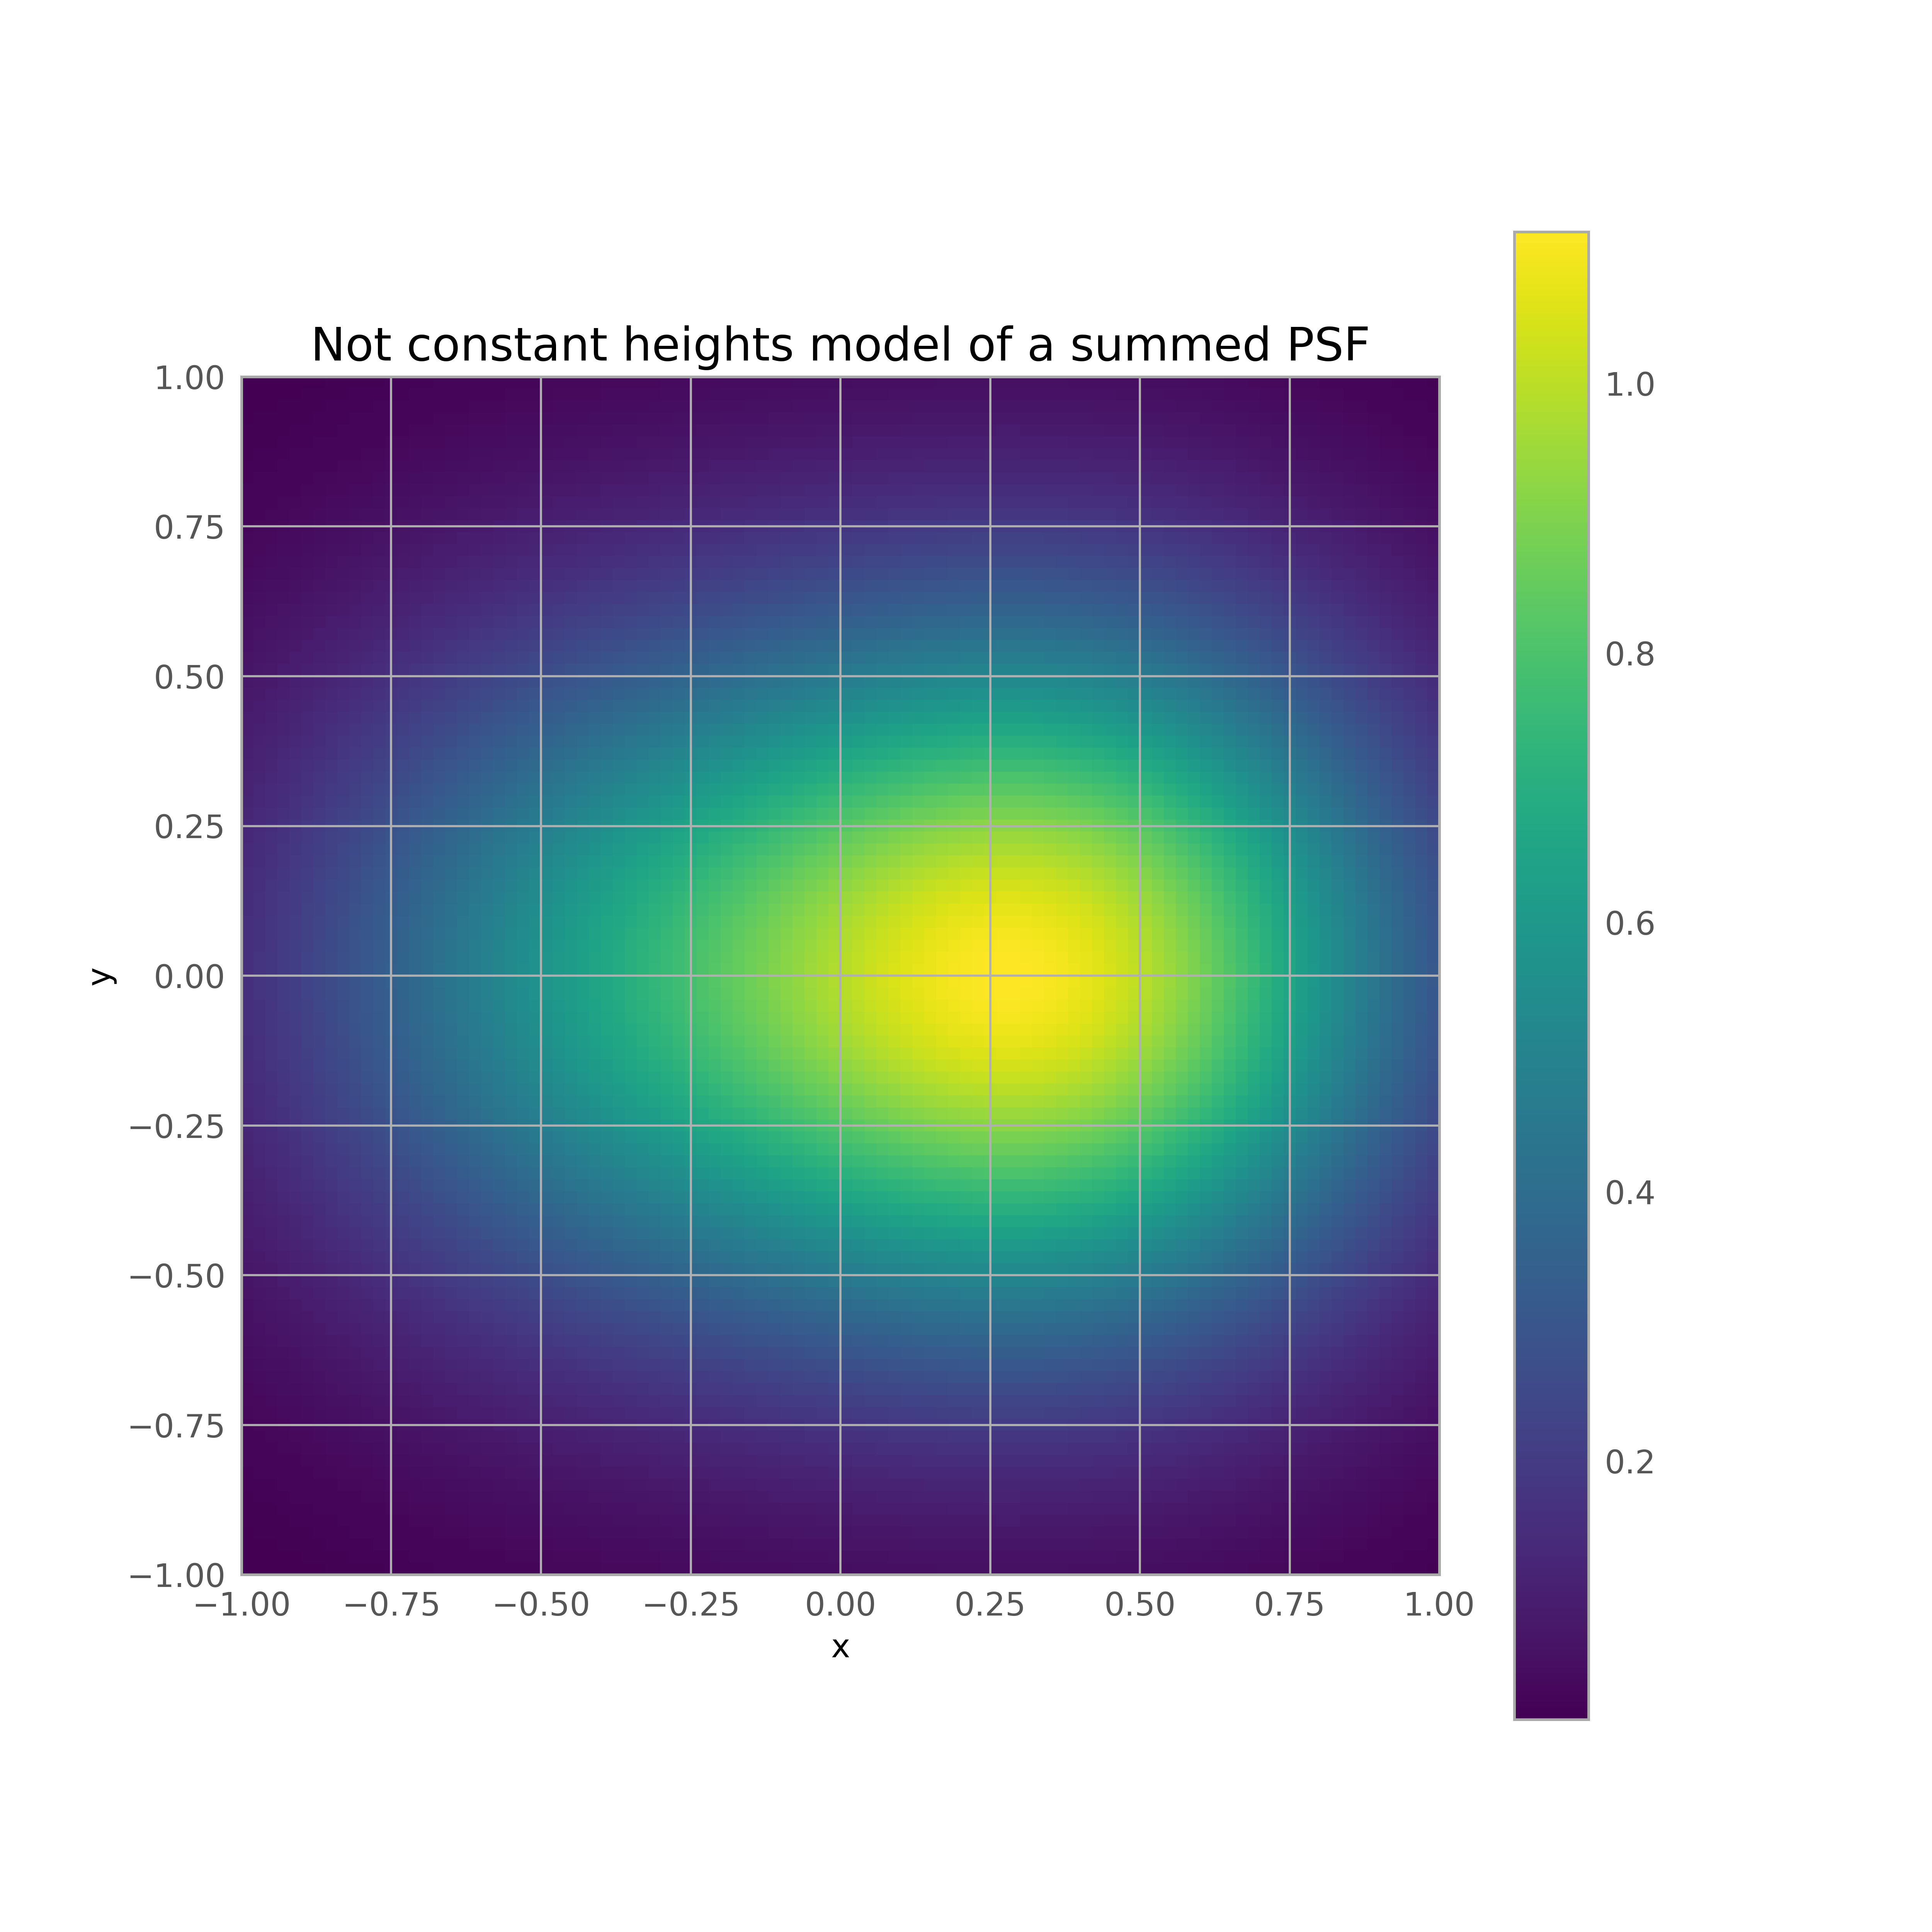
\includegraphics[width=\textwidth]{report/Figures/models/model_psf_notconst.png}
        \end{subfigure}%
        \hspace{1em}-
        \begin{subfigure}{.45\textwidth}
            \centering
            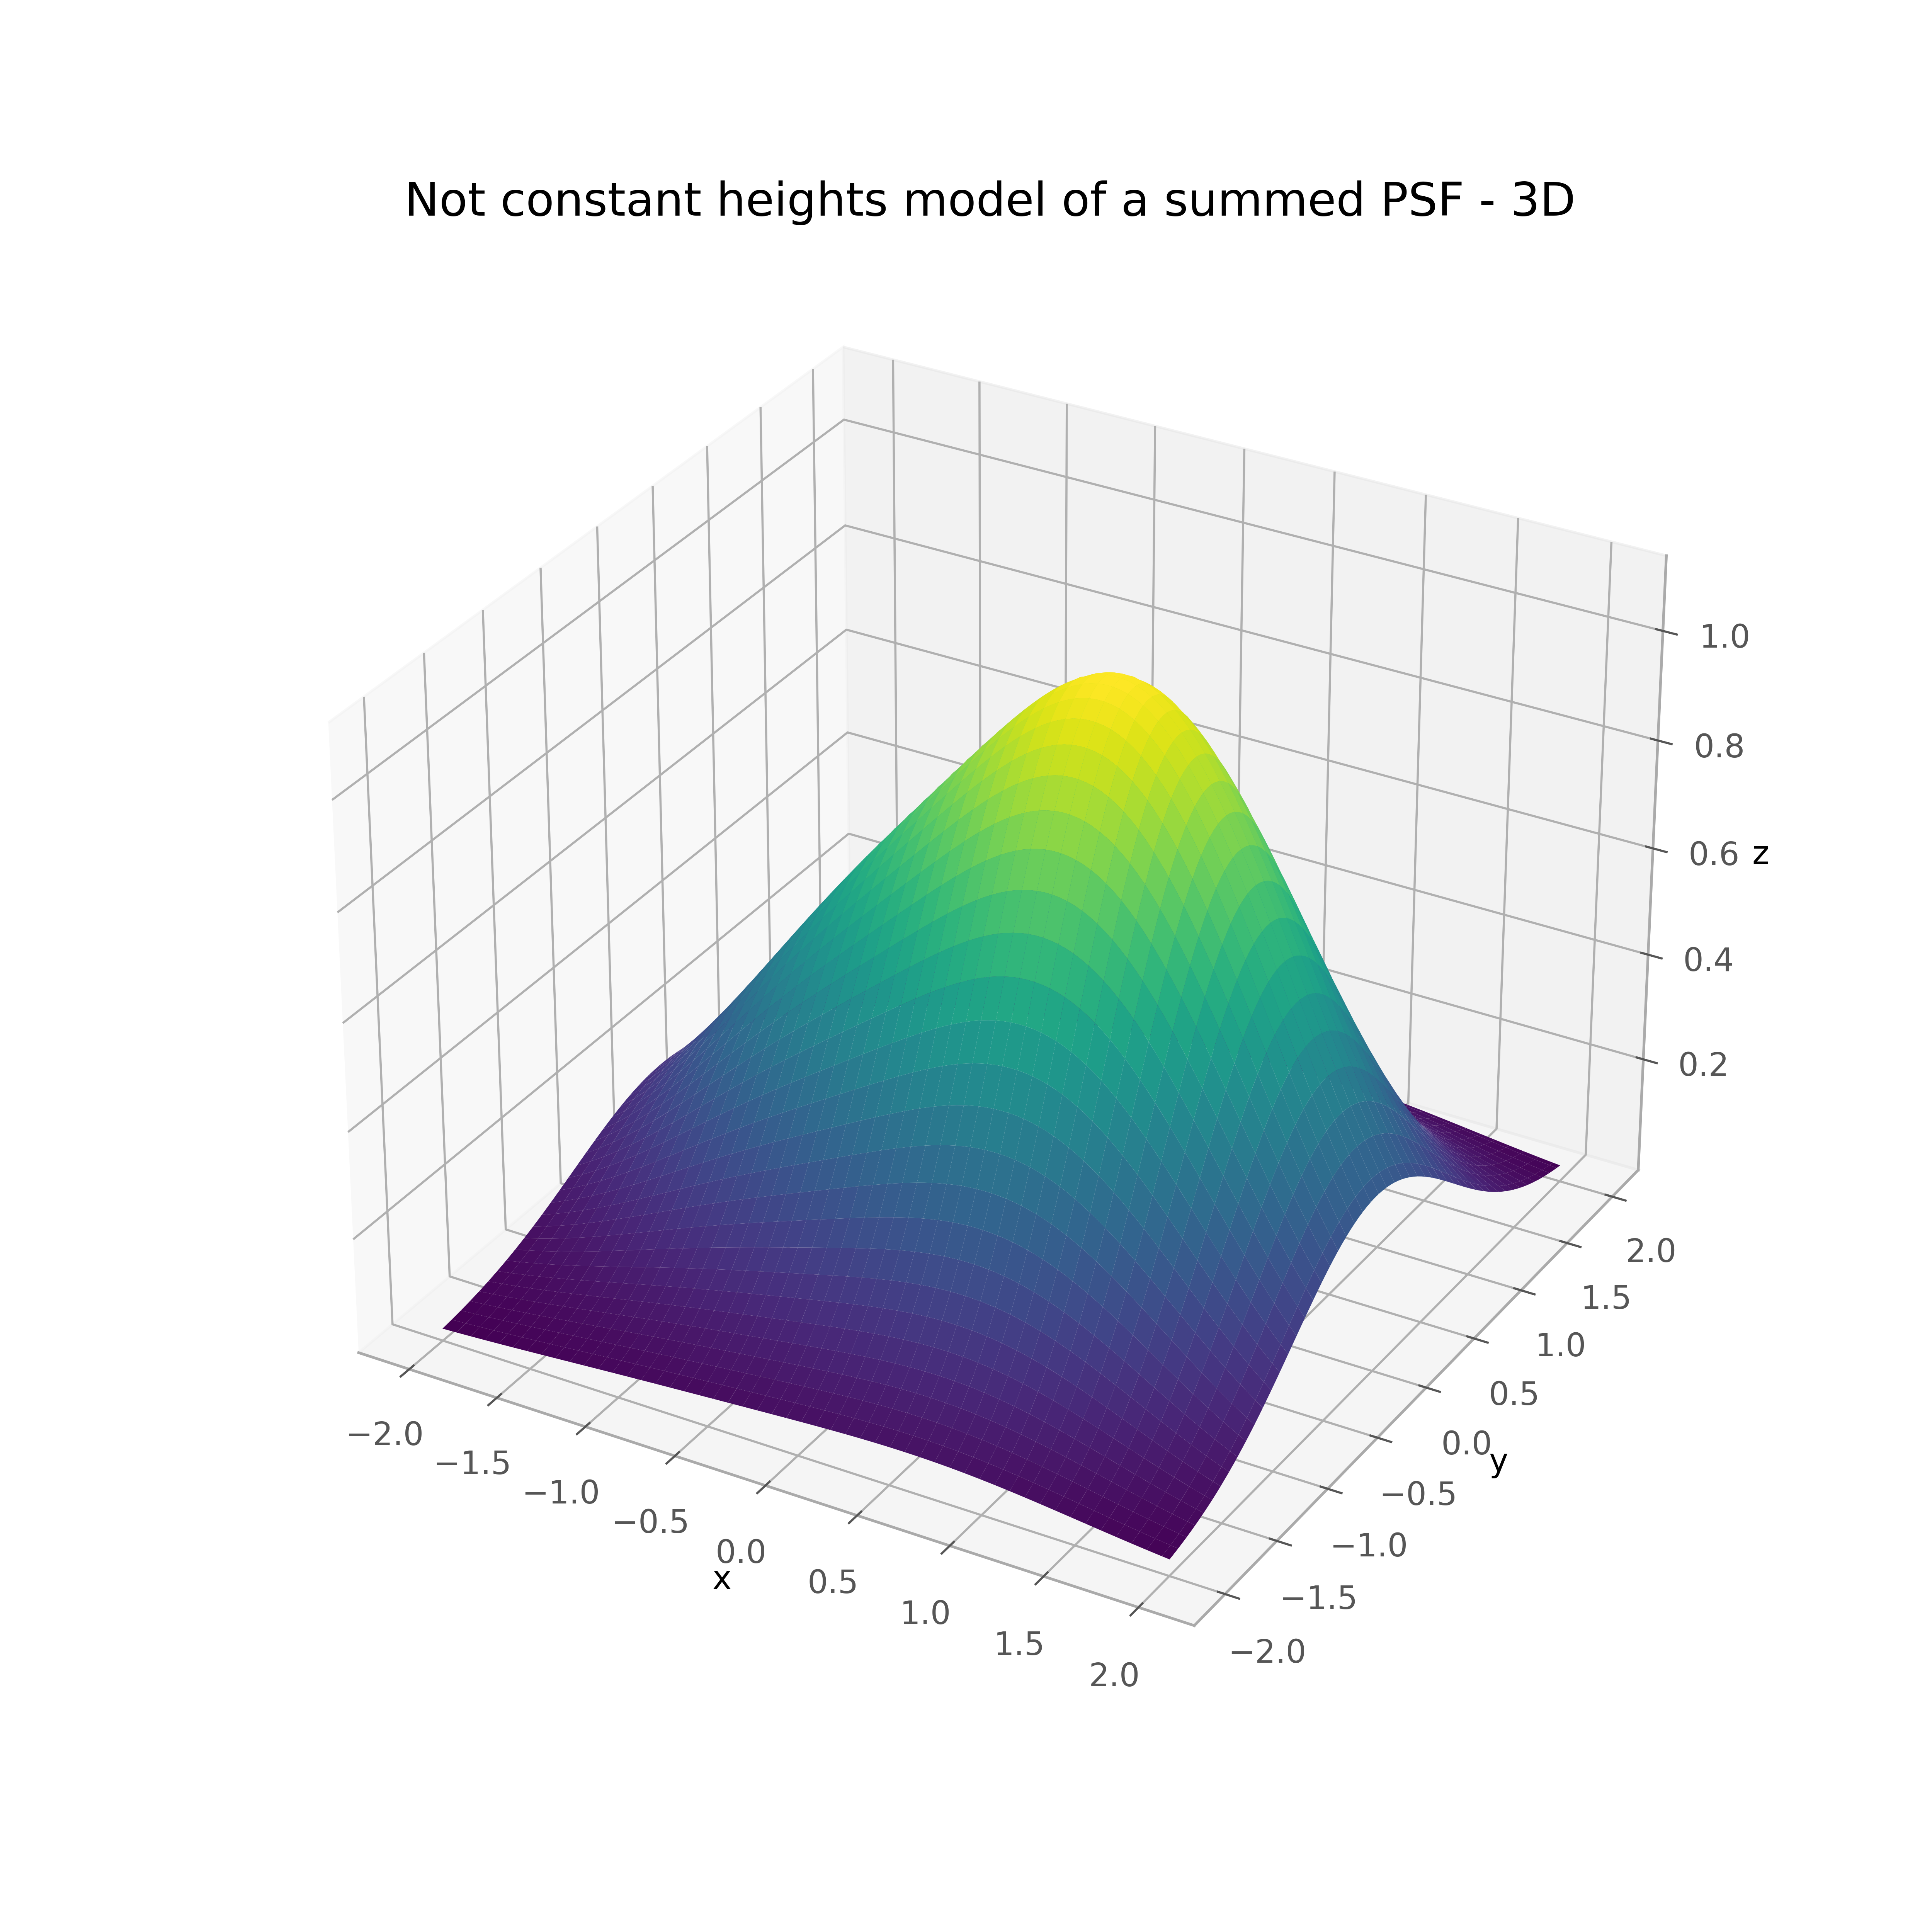
\includegraphics[width=\textwidth]{report/Figures/models/model_psf_notconst_3d.png}
        \end{subfigure}
        \caption{Non constant summed PSFs used as models for Venus' flux.}
        \label{model_psf_notconst}
        \end{figure}

        \begin{figure}[H]
        \centering
        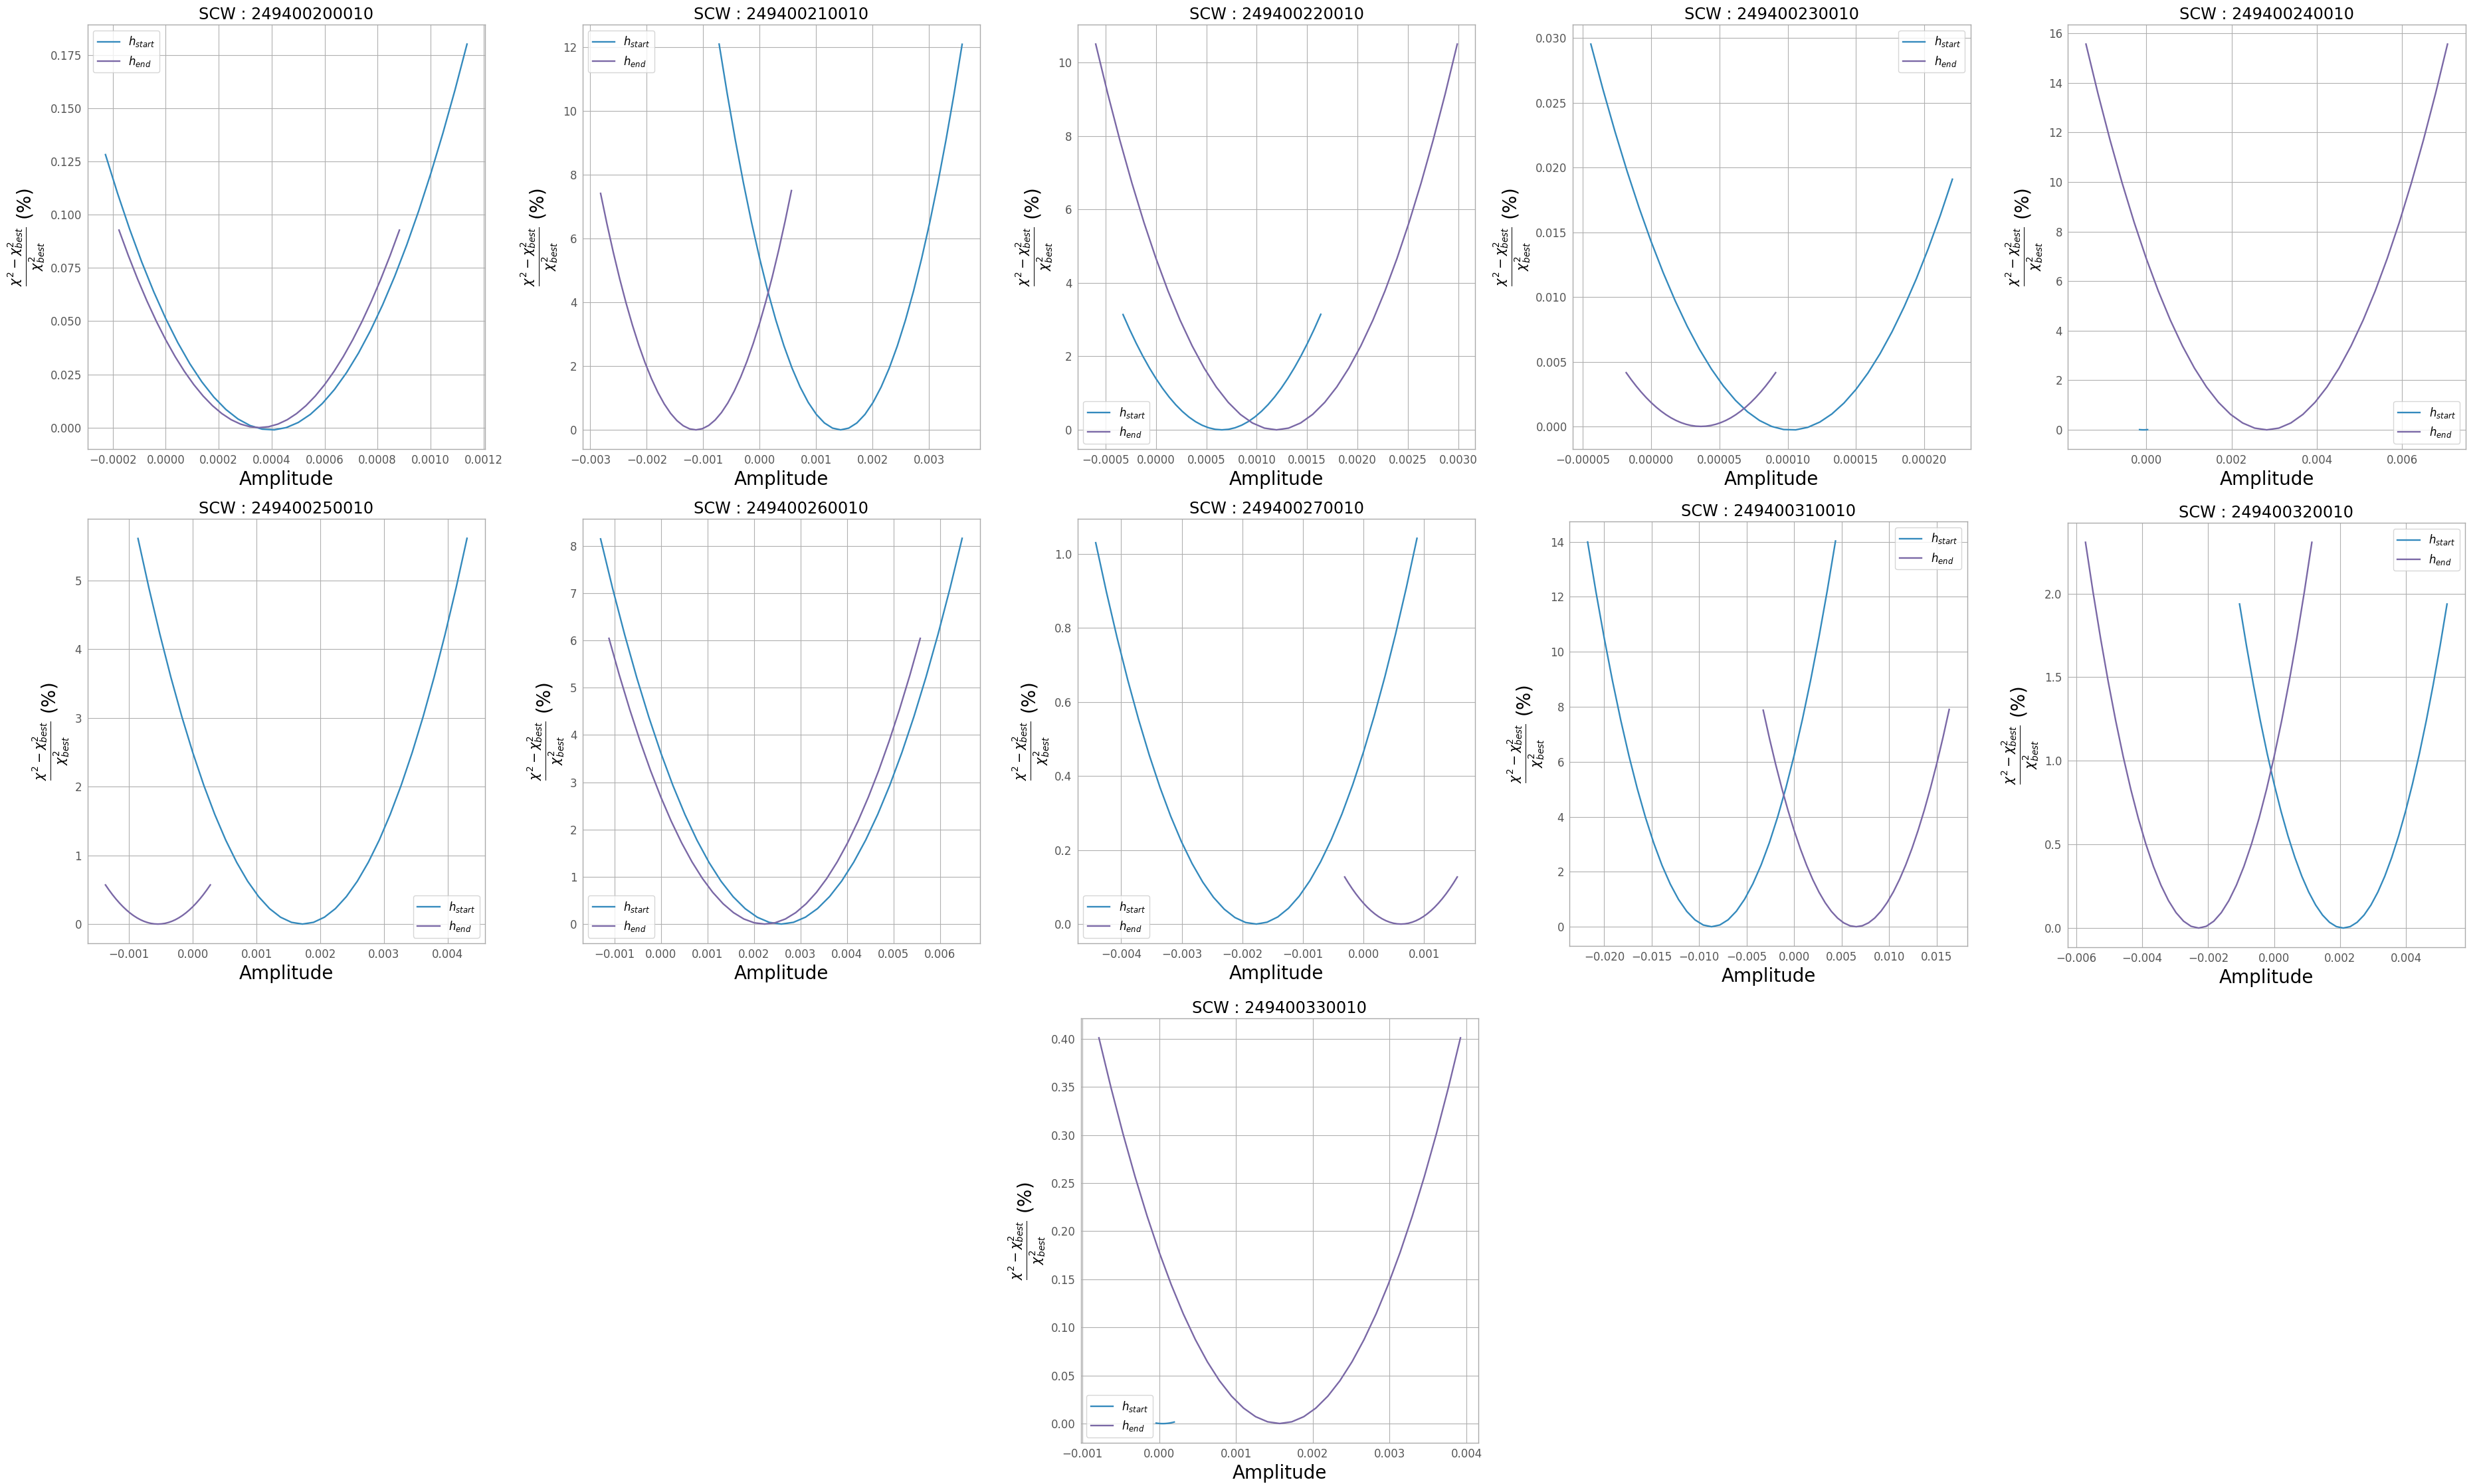
\includegraphics[width = \textwidth]{report/Figures/models/2204/threshold_determination_notconst.png}
        \caption{Normalised deviations from the optimised height for each flux point. The threshold is set at 2\% of the best-fit value.}
        \label{threshold}
        \end{figure}

    
    %--------------------------------------------------
    
    \subsection{Solar events}
    
    \begin{figure}[H]
        \centering
        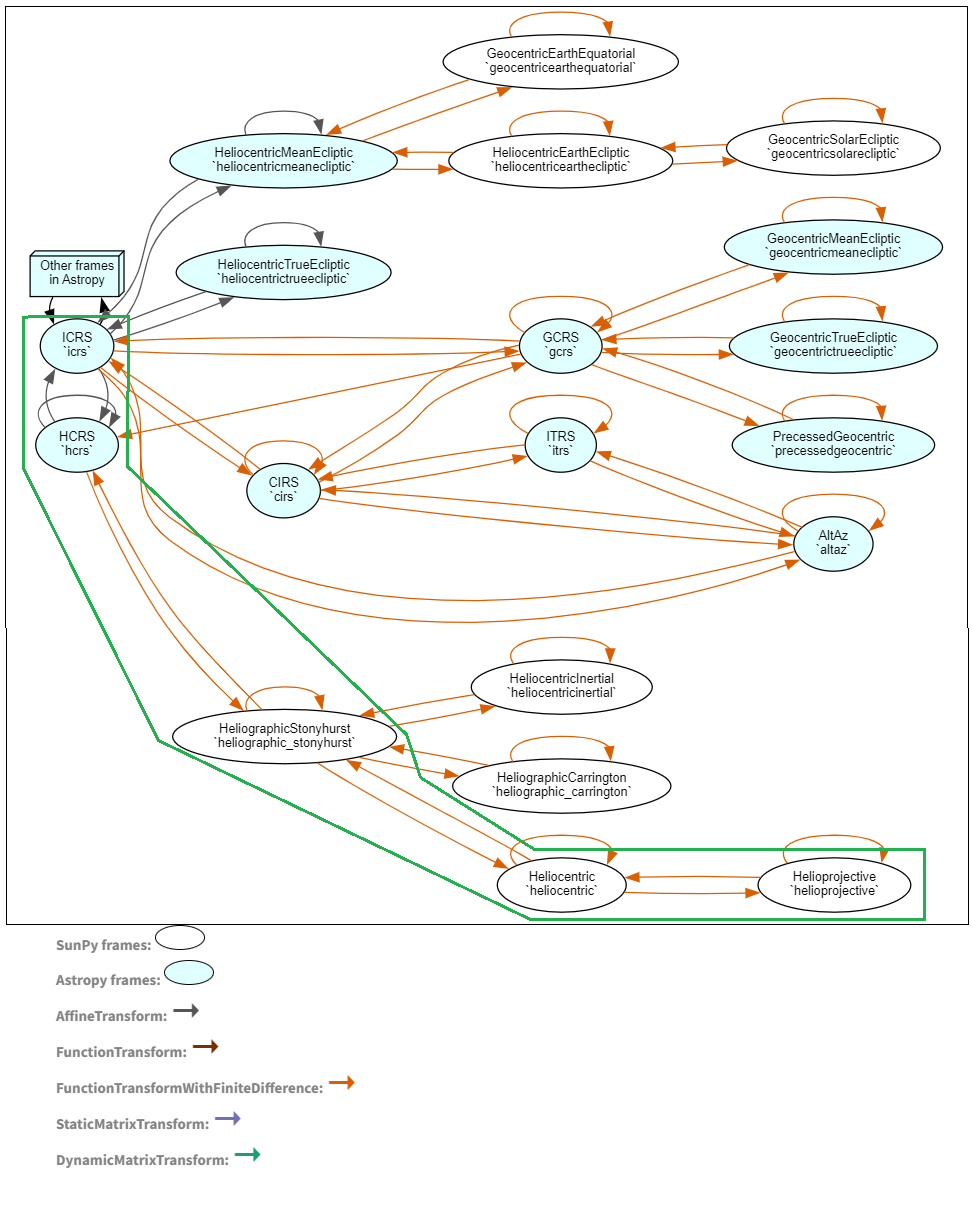
\includegraphics[width = 12cm]{report/Figures/methods/coordinates.png}
        \caption{\texttt{Sunpy} and \texttt{Astropy} coordinate frames transformations. The path used for this study is boxed in green.}
        \label{coordinates}
    \end{figure}

    \begin{figure}[H]
        \centering
        
\includegraphics[width = \textwidth]{report/Figures/methods/GOES_total.png}
        \caption{Solar flux in the XRSA channel(1.5-12.4 keV) of the GOES-16 spacecraft from the 19.04.2022 to the 24.04.2022. The solar flare classes are delimited on the right of each plot.}
        \label{goes_tot}
    \end{figure}